\documentclass[11pt,a4paper]{report}

\usepackage[portuges]{babel}
\usepackage[utf8]{inputenc} % define o encoding usado texto fonte (input)--usual "utf8" ou "latin1
\usepackage{graphicx} %permite incluir graficos, tabelas, figuras
\usepackage{subcaption}
\usepackage[title]{appendix}
\usepackage{listings}
\usepackage{color}
\usepackage{multicol}
\usepackage{indentfirst}
\usepackage{hyperref}
\usepackage{amsmath}
\usepackage{amssymb}
\usepackage{float}
\usepackage[inline]{enumitem}


\definecolor{mygreen}{rgb}{0,0.6,0}
\definecolor{mygray}{rgb}{0.5,0.5,0.5}
\definecolor{mymauve}{rgb}{0.58,0,0.82}

\lstset{ %
  backgroundcolor=\color{white},   % choose the background color
  basicstyle=\footnotesize,        % size of fonts used for the code
  breaklines=true,                 % automatic line breaking only at whitespace
  captionpos=b,                    % sets the caption-position to bottom
  commentstyle=\color{mygreen},    % comment style
  escapeinside={\%*}{*)},          % if you want to add LaTeX within your code
  keywordstyle=\color{blue},       % keyword style
  stringstyle=\color{mymauve},     % string literal style
}

\title{Processamento de Linguagens e Compiladores - Trabalho Prático 1\\
       \textbf{Grupo 3}\\ Relatório
       } %Titulo do documento
%\title{Um Exemplo de Artigo em \LaTeX}
\author{Alef Pinto Keuffer\\ (A91383)\and Catarina Martins Sá Quintas \\ (A91650)\and  Ivo Miguel Gomes Lima \\(A90214)
       } %autores do documento
\date{\today} %data

\begin{document}
	\begin{minipage}{0.9\linewidth}
        \centering
		
\includegraphics[width=0.4\textwidth]{um.jpeg}\par\vspace{1cm}
                \href{https://www.uminho.pt/PT}
		{\scshape\LARGE Universidade do Minho} \par
		\vspace{0.6cm}
                \href{https://lcc.di.uminho.pt}
		{\scshape\Large Licenciatura em Ciências da Computação} \par
		\maketitle
	\end{minipage}

\tableofcontents % insere Indice

\chapter{Introdução}


No âmbito da unidade curricular Processamento de Linguagens e compiladores (PLC),
foi-nos proposto a realização de um projeto de forma a aprofundar os nossos
conhecimentos adquiridos na sala de aula, atingindo os seguintes objetivos:

\begin{itemize}
    \item Aumentar a capacidade de escrever Expressões Regulares(ER)
    \item Desenvolver sistematicamente Processadores de Linguagens Regulares, ou Filtros de Texto.
    \item Familiarizar com o módulo 're' presente no Python.
\end{itemize}
  

Para o efeito, criamos um  processador de Bib\TeX \href{http://www.bibtex.org/}. 
A Bib\TeX \ é uma ferramenta de formatação usada em documentos em La\TeX.
Um exemplo desta ferramenta pode ser visto abaixo: 
\begin{lstlisting}
@techreport{jspell1,
   author = "J.J. Almeida and Ulisses Pinto",
   title = "Manual de Utilizador do {JSpell}",
   year = 1994,
   type = "Manual",
   month = "Jul",
   institution = "umdi",
   keyword = "morphology, lexical analysis,jspell",
   abstract = {},
   url = "http://natura.di.uminho.pt/~jj/pln/jspellman.ps.gz",
}

\end{lstlisting}

Existe um conjunto de campos obrigatórios e facultativos para que um Bib\TeX \ seja válido, alguns desses campos são: \emph{article}, \emph{book}, \emph{inproceedings}, \emph{misc}, \emph{proceedings} entre outros.



\newpage

\section{Descrição do Problema}
\subsection{Especificação dos Requisitos }

\newcommand{\gv}{\emph{GraphViz}}
\newcommand{\htlm}{\emph{HTML}}
\newcommand{\dott}{\emph{Dot}}
\newcommand{\bib}{Bib\TeX}



A nossa solução deve satisfazer os seguintes requisitos: 
\begin{enumerate}[label=R\arabic*]
\item\label{R1} Fazer a contagem das categorias presentes no documento, tais como: \emph{phDThesis}, \emph{Misc}, \emph{InProceeding }, \emph{etc }.
\item\label{R2}Produzir um documento em formato \htlm \ com
\begin{enumerate*}[label=(R2.\arabic*)]
  \item\label{R21} o nome das categorias encontradas e
  \item\label{R22} respectivas contagens.
\end{enumerate*}
\item\label{R3} Filtrar, para cada entrada de cada categoria, a respetiva
\begin{enumerate*}[label=(R3.\arabic*)]
  \item\label{R31} chave
  \item\label{R32} autores,
  \item\label{R33} e título.
  \item\label{R34} O resultado final deverá ser incluído no documento \htlm \ gerado \ref{R2}.
\end{enumerate*}

\item\label{R4} Criar um índice de autores, que mapeie cada autor nos respectivos registos, de modo a que posteriormente uma ferramenta de procura do Linux possa fazer a pesquisa.

\item\label{R5} Construir um Grafo que mostre, para um dado autor (definido à partida) todos os autores que publicam normalmente com o autor em causa.
\item\label{R6}Recorrendo à linguagem \dott \  do \gv, gerar um ficheiro com o grafo de \ref{R5} de modo a que possa, posteriormente, usar uma das ferramentas que processam \dott \  para desenhar o dito grafo de associações de autores.
\end{enumerate}

\chapter{Concepção de Resolução }
\section{Tarefa 4 a}

A estratégia para satisfazer \ref{R1} consistiu em ler o arquivo linha a linha verificando se a categoria encontrada já aparecia no dicionário, se já existir, irá ser incrementado o número de ocorrências, senão será adicionado como primeira ocorrência, para que depois possa ser produzido um ficheiro \htlm\ com todas as categorias e o devido número de ocorrências.

\subsubsection{Expressão Regular}
De seguida apresentamos a Expressão Regular utilizada para filtrar a informação pedida em \ref{R1}.

Uma vez que todas as categorias num \bib\ têm como antecedente o caráter @ e terminam numa \{, tornou-se fácil criar um filtro que guarde toda a informação delimitada entre esses dois parâmetros.

Através dessa pequena realização chegamos à seguinte expressão: \textbf{$\land$@(.*)\{}

\newpage
\subsubsection{Implementação}
\begin{lstlisting}[language=python]
import re

file = open("exemplo-utf8.bib", "r")
read = True
dic = {}
string_ls = ['<!DOCTYPE  HTML PUBLIC>\n<HTML>\n   <HEAD>\n      <TITLE>Categories in BibTeX</TITLE>\n   </HEAD>\n   <BODY>']
while read:
    linhaFicheiro = file.readline()
    ncat = re.match(r'^@(.*){',linhaFicheiro)
    if ncat != None:
       cat_title = ncat.group(1).title()
       dic[cat_title] = dic.get(cat_title,0) + 1
    if not linhaFicheiro:
       read = False
       file.close()

time = lambda v: 's' if v > 1 else ''

for k, v in dic.items():
    string_ls.append(f'      <P>The category {k} appears {v} time{time(v)}.</P>')
    string_ls.append(f'   </BODY>\n</HTML>')
with open('output.html','w') as file:
     file.write('\n'.join(string_ls))
\end{lstlisting}

\section{Resultado}

\begin{figure}[h]
\centering
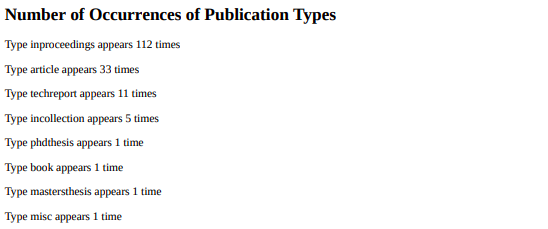
\includegraphics[width=1.2\textwidth]{P/categoriesNumber.jpeg}
\caption{Número de Ocorrências das Categorias}
\end{figure}
\newpage
\section{Tarefa 4 b}

\subsubsection{Algoritmos}

Infelizmente a estratégia adotada na primeira questão de unicamente guardar aquilo que interessava tornou-se impraticável pois os parâmetros pedidos nas outras questões não tinham tanta consistência, ou seja, podiam estar envolvidos \{\} entre \{\}, podiam alterar a ordem pela qual apareciam, entre outros contratempos.

Portanto começamos a associar os pares de (tipo da publicação, chave) com os campos da entrada e aplicar diversas manipulações sobre essa estrutura de modo a satisfazer os requisitos.

Para o efeito utilizamos vários algoritmos de agrupamento e filtragem da informação pretendida de modo a conseguir converter o ficheiro \bib\ num ficheiro \emph{HTML}.

Todos os algoritmos tem a sua função explicitada abaixo, sendo cada um destes fundamental para a execução do programa:

\begin{itemize}
    \item get\_bib\_str: Abre \bib
    \item get\_pub\_type\_counts: Conta e enunciar categorias
    \item get\_entries: Copia todos os dados \bib para um dic
    \item get\_valid\_group: Guarda título, nome e chave todos os que aparece entre " " ou em \{\}
    \item  unbrace: Retirar \{\} dentro de \{\} ou seja \{\{cenas\}\} = cenas
    \item get\_author\_list: Ordena autores alfabeticamente para ser mais fácil filtrar
    \item invert\_name: exemplo: da Cruz, Daniela -> Daniela da Cruz
    \item remove\_latex\_special\_chars: Transforma serif, small caps,... 
    \item html\_create\_span: Coloca o <SPAN> ... </Span>
    \item html\_enclose:  Coloca as <cenas> ... </cenas>
    \item html\_to\_small\_caps: Coloca o texto assim
    \item  html\_to\_sans\_serif: Coloca o texto assim
    \item  html\_add\_attr: colocar um atributo exemplos de cima
    \item get\_html\_pub\_type\_index: Mudifica as entradas colocando mais atributos html
    \item get\_html\_pub\_type\_index: Mudifica as entradas colocando mais atributos html
    \item str\_to\_html\_math: Processa expressões matemáticas
    \item fix\_title: Faz busca dos atributos que tem de ser mudados enviando para a função que as realiza
    \item fix\_repeated\_authors: Faz a junção de autores que sao a mesma pessoa
    \item format\_authors: Escolhe remover acentuações e caracteres especiais  que as representam em latex (e.g. "\\~") do nome dos autores.
    \item remove\_consecutive\_spaces: Remover os espaços consecutivos 
    \item remove\_latex\_accent: Remove os acentos em latex 
    \item last\_name\_first: Recebe um nome normalizado (e.g. Pedro Filipe H. Pereira) e deve retornar "invertido" (e.g. Pereira, P. F. H.)
    \item is\_a\_first\_last\_match: Verifica 1 letra autor 1 com 1 letra autor 2 e o mesmo para a segunda
    \item get\_crude\_abbrev: Coloca todos os nomes a maiuscula
    \item is\_a\_first\_last\_match: Verifica se a letra do primeiro autor e igual a 1 letra do segundo autor e o mesmo para a 2 letra  
    \item block\_authors\_with\_two\_common\_names\_v2: Cria blocos com nomes dos autores, quem estiver no mesmo bloco, e a mesma pessoa.
    \item fix\_block\_func: Cria transitividade nos autores.  Sem essa função, temos blocos {A,B} e {B,C} Depois dessa função, vamos ter {A,B,C}
    \item get\_html\_pub\_type\_counts: Coloca  em formato \htlm parâmetros utilizados em \ref{R2}
    \item mult\_replace: Muda o posicionamento dos nomes atraves de uma lista em regex
    
    
\end{itemize}
\newpage
\subsubsection{Expressões Regulares}

De seguida iremos apresentar as Expressões Regulares utilizadas para normalizar o texto presente no \bib\ e filtrar as informações relevantes:
\begin{itemize}
\item Para capturar tudo os que está dentro das 
\begin{lstlisting}
\b}
\end{lstlisting}
\item Esta expressão é útil para
\begin{lstlisting}
(\w+)\s*=\s*(?:{((?:[^{}]+|{(?:[^{}]+|{[^{}]*})+})+)}|"([^"]+)"|(\d+))
@(\w+){(.+),((?:[^{}]+|{(?:[^{}]*|{[^{}]*})+})+)
\end{lstlisting}
\item Substituir nomes:
\begin{lstlisting}
([^,]+),\s*([^,]+) ... \2 \1
\end{lstlisting}
\item Esta expressão é útil para
\begin{lstlisting}
\\({|[^{])\b
\end{lstlisting}
\item Usamos esta expressão com o intuito de 
\begin{lstlisting}
<(\w+)([^>]*)\s*>(.*)</\1> .... <\1\2 {attr.upper()}="{val}">\3</\1>
\end{lstlisting}
\item Expressão utilizada para
\begin{lstlisting}
\\textsc{((?:\\{|[^{])+)}
\end{lstlisting}
\item Esta expressão é útil para
\begin{lstlisting}
\band\b
\end{lstlisting}
\item A expressão abaixo apresentada serve para 
\begin{lstlisting}
\s+
\end{lstlisting}
\item Abaixo apresentamos a expressão que 
\begin{lstlisting}
\\\W
\end{lstlisting}
\item Nesta expressão
\begin{lstlisting}
\w\w+
\end{lstlisting}
\end{itemize}

\subsubsection{Implementação}
\begin{lstlisting}[language=python]
import re
import unicodedata

HTML_PROLOGUE = '<!DOCTYPE  html>\n<HTML lang="en">\n<HEAD>\n<meta charset="utf-8">\n      <TITLE>Categories in BibTeX</TITLE>\n <script type="text/x-mathjax-config"> MathJax.Hub.Config({"extensions":["tex2jax.js"],"jax":["input/TeX","output/HTML-CSS"],"messageStyle":"none","tex2jax":{"processEnvironments":false,"processEscapes":true,"inlineMath":[["$","$"],["\\(","\\)"]],"displayMath":[["$$","$$"],["\\[","\\]"]]},"TeX":{"extensions":["AMSmath.js","AMSsymbols.js","noErrors.js","noUndefined.js"]},"HTML-CSS":{"availableFonts":["TeX"]}}); </script> <script type="text/javascript" async src="file:////home/useralef/.vscode/extensions/shd101wyy.markdown-preview-enhanced-0.6.1/node_modules/@shd101wyy/mume/dependencies/mathjax/MathJax.js" charset="UTF-8"></script>  </HEAD>\n'
HTML_EPILOGUE = '</HTML>'
BIB_EXAMPLE_FILENAME = "exemplo-utf8.bib"
OUTPUT_FILENAME = 'output.html'

#abrir bibtex
def get_bib_str(filename):
    with open(filename,'r') as file:
        return re.sub(r'\b}',r' }',file.read())

#contar e enunciar categorias
def get_pub_type_counts(data):
    pub_types_occur = [x[0] for x in data.keys()]
    pub_types = set(pub_types_occur)
    return [(pub_type, pub_types_occur.count(pub_type)) for pub_type in pub_types]

#copiar todos os dados bib para um dic {field:field_value}
def get_entries(string):
    d = {}
    field = re.compile(r'(\w+)\s*=\s*(?:{((?:[^{}]+|{(?:[^{}]+|{[^{}]*})+})+)}|"([^"]+)"|(\d+))')
    for entry in re.finditer(r"@(\w+){(.+),((?:[^{}]+|{(?:[^{}]*|{[^{}]*})+})+)", string):
        d[entry.group(1).lower(), entry.group(2)] = {
            x[0].lower(): get_valid_group(x, 1, 3)
            for x in field.findall(entry.group(3))}
    return d

#Guardar titulo,nome,chave todos os que aparece entre " " ou em {}
def get_valid_group(t, begin_or_group, end_or_group):
    for i in range(begin_or_group, end_or_group + 1):
        if v := t[i]:
            return v

# Retirar {} dentro de {} ou seja {{cenas}} = cenas
def unbrace(expression):
    return expression.translate({ord(x):None for x in '{}'})

#Ordenar autores alfabeticamente para ser mais facil filtrar
def get_author_list(data):
    return sorted(set([a for s in data.values() for a in s.get("author", [])]))

#Por exemplo: da Cruz, Daniela -> Daniela da Cruz
def invert_name(author_name):
    return re.sub(r"([^,]+),\s*([^,]+)", r"\2 \1", author_name)

# Transformar serif, small caps,... 
def remove_latex_special_chars(latex_expression):
    return re.sub(r'\\({|[^{])\b',r'\1',latex_expression)

#Por o <SPAN> ... </Span>
def html_create_span(expression):
    return html_enclose('span',expression)

#Por as <cenas> ... </cenas>
def html_enclose(tag,string):
    return rf'<{tag.upper()}>{string}</{tag.upper()}>'

# Colocar o texto assim https://www.w3schools.com/cssref/tryit.asp?filename=trycss_font-variant
def html_to_small_caps(html_expression):
    return html_add_attr('style','font-variant:small-caps',html_expression)

#colocar o texto assim https://www.w3schools.com/cssref/tryit.asp?filename=trycss_font-family
def html_to_sans_serif(html_expression):
    return html_add_attr('style','font-family:sans-serif',html_expression)

#colocar um atributo exemplos de cima
def html_add_attr(attr,val,html_expression):
    return re.sub(r'<(\w+)([^>]*)\s*>(.*)</\1>',rf'<\1\2 {attr.upper()}="{val}">\3</\1>',html_expression)

# mudifica as entradas colocando mais atributos html
def get_html_pub_type_index(data):
    string_ls = [html_enclose('h2','Publication Type Index')]
    for entry_type in sorted(set(x[0] for x in data)):
        string_ls.append(html_enclose('h3',entry_type))
        for citation_key in [x[1] for x in data if x[0]==entry_type]:
            title = data[entry_type,citation_key].get('title','')
            authors = ', '.join((sorted(data[entry_type,citation_key].get('author',''))))
            string_ls.append(html_enclose('p',f"Key = {citation_key}<br>Title = {fix_title(title)}<br>Autores = {authors}"))
    return '\n'.join(string_ls)

#Processar expressoes matematicas
def str_to_html_math(string):
    return html_add_attr('class','math inline',html_create_span(string))

#faz busca dos atributos que tem de ser mudados enviando para a funcao que as realiza
def fix_title(title):
    substitutions = [(r'\\textsc{((?:\\{|[^{])+)}',lambda m: f'{html_to_small_caps(html_create_span(m.group(1)))}'),
                     (r'\\textsf{((?:\\{|[^{])+)}',lambda m: f'{html_to_sans_serif(html_create_span(m.group(1)))}'),
                     (r'(\$(?:.|\\\$)+\$)', lambda m: f'{str_to_html_math(m.group(1))}')]


    replace = lambda x: mult_replace(x,substitutions)

    return   html_create_span(
             unbrace(
             replace(
             remove_latex_special_chars(
             remove_accents(
             ' '.join(s.strip() for s in title.split('\n')))))))

#Faz a juncao de autores que sao a mesma pessoa
def fix_repeated_authors(data):
    author_blocks = fix_block_func(block_authors_with_two_common_names_v2(get_author_list(data)))
    author_dict = {author_name:max(s,key=len) for s in author_blocks for author_name in s}
    for d in data.values():
        d['author'] = [author_dict[author] for author in d['author']]

# Escolhemos remover acentuacoes e caracteres especiais  que as representam em latex (e.g. "\\~") do nome dos autores.
def format_authors(data):
    for d in data.values():
        if "author" in d:
            author_lst = [ remove_consecutive_spaces(
                           str.strip(
                           invert_name(
                           unbrace(
                           remove_accents(name)))))
                           for name in re.split(r"\band\b", d["author"].replace("\n", " "))]
            d['author'] = [author for author in author_lst if author]


def remove_consecutive_spaces(name):
    return re.sub(r'\s+',' ',name)

def remove_latex_accent(name):
    return re.sub(r'\\\W','',name)

def remove_normal_accent(name):
    return ''.join((c for c in unicodedata.normalize('NFD', name) if unicodedata.category(c) != 'Mn'))

# Recebe um nome normalizado (e.g. Pedro Filipe H. Pereira) e deve retornar "invertido" (e.g. Pereira, P. F. H.)
def last_name_first(name):
    initials =  '. '.join(get_crude_abbrev(name))[:-2]
    last_name = name.split()[-1]
    return f'{last_name}, {initials}'

#Verificar 1 letra autor 1 com 1 letra autor 2 e o mesmo para a segunda
def is_a_first_last_match(author1,author2):
    a1 = get_crude_abbrev(author1)
    a2 = get_crude_abbrev(author2)
    return a1[0] == a2[0] and a1[-1] == a2[-1]

# colocar todos os nomes a maiuscula
def get_crude_abbrev(name):
    return ''.join(c for c in name if c.isupper())

# Verificar se a letra do primeiro autor e igual a 1 letra do sengundo autor e o mesmo para a 2 letra 
def is_a_first_last_match(author1,author2):
    a1 = get_crude_abbrev(author1)
    a2 = get_crude_abbrev(author2)
    return a1[0] == a2[0] and a1[-1] == a2[-1]

# Criar blocos com nomes dos autores, quem estiver no mesmo bloco, e a mesma pessoa.
def block_authors_with_two_common_names_v2(authors):
    res = set()
    for author in authors:
        fs = set()
        for author2 in authors:
            a1 = set(re.findall(r'\w\w+',author))
            a2 = set(re.findall(r'\w\w+',author2))
            if len(a1.intersection(a2)) > 1:
                fs.add(author2)
            elif len(a1) == 1 and len(a1.intersection(a2)) == 1 and is_a_first_last_match(author,author2):
                fs.add(author2)
        res.add(frozenset(fs))
    return res

#Criar transitividade nos autores.  Sem essa funcao, temos blocos {A,B} e {B,C} Depois dessa funcao, vamos ter {A,B,C}
def fix_block_func(data):
    res = set()
    for s1 in data:
        q = s1.copy()
        for s2 in data:
            if s1.intersection(s2) != set():
                q = q.union(s2)
        res.add(frozenset(q))
    return res

def get_html_pub_type_counts(data):
    string_ls = [html_enclose('h2','Number of Occurrences of Publication Types')]
    pub_counts = sorted(get_pub_type_counts(data),key=lambda x: x[1],reverse=True)
    time = lambda v: 's' if v > 1 else ''
    for pub_type, count in pub_counts:
        string_ls.append(html_enclose('p',f'Type {pub_type} appears {count} time{time(count)}'))
    return ''.join(string_ls)

#muda o posicionamento dos nomes atraves de uma lista em regex
def mult_replace(string, replacement_list):
    for old, new in replacement_list:
        string = re.sub(old, new, string)
    return string

# Função mais importante que inicializa tudo
def solve(author_name,INPUT_FILENAME=BIB_EXAMPLE_FILENAME):
    html_str_ls = [HTML_PROLOGUE]
    bib_str = get_bib_str(INPUT_FILENAME)

    entries = get_entries(bib_str)
    format_authors(entries)
    fix_repeated_authors(entries)

    html_str_ls.append(html_enclose('body',f'{get_html_pub_type_counts(entries)}{get_html_common_pub_author(author_name,entries)}{get_html_pub_type_index(entries)}{get_html_author_index(entries)}'))

    html_str_ls.append(HTML_EPILOGUE)

    with open(OUTPUT_FILENAME,'w') as file:
        file.write('\n'.join(html_str_ls))

\end{lstlisting}

\subsection{Resultado}

\begin{figure}[h]
\centering
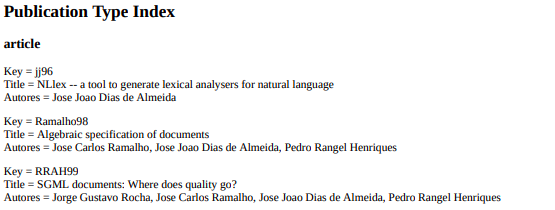
\includegraphics[width=1.2\textwidth]{P/categoriesAndauthors.jpeg}
\caption{Índice do Tipo de Publicação}
\end{figure}

\section{Tarefa 4 c}

\subsubsection{Implementação}
\begin{lstlisting}[language=python]

#faz a juncao de todos os autores no bib para o dicionario aplicando lhe um primeiro filtro
def get_author_index_dict(data):
    index = {}
    for key, e in data.items():
        if 'author' in e:
            for author in e['author']:
                author_name = last_name_first(author)
                if author_name not in index:
                    index[author_name] = set()
                index[author_name].add(key[1])
    return index

#Faz a transformacao de os autores no bib para ficarem no html 4 c
def get_html_author_index(data):
    index = sorted(get_author_index_dict(data).items())
    alphabet_order = sorted(set(c[0][0] for c in index))
    string_ls = [html_enclose('h2','Author Index')]
    i = 0
    string_ls.append(html_enclose('h3',alphabet_order[i]))
    for author,citation_keys in index:
        if author[0] != alphabet_order[i]:
            i += 1
            string_ls.append(html_enclose('h3',alphabet_order[i]))
        citation_keys_str = ', '.join(citation_keys)
        string_ls.append(html_enclose('p',f'{author}, {citation_keys_str}'))
    return ''.join(string_ls)
\end{lstlisting}

\subsection{Resultado}
\begin{figure}[h]
\centering
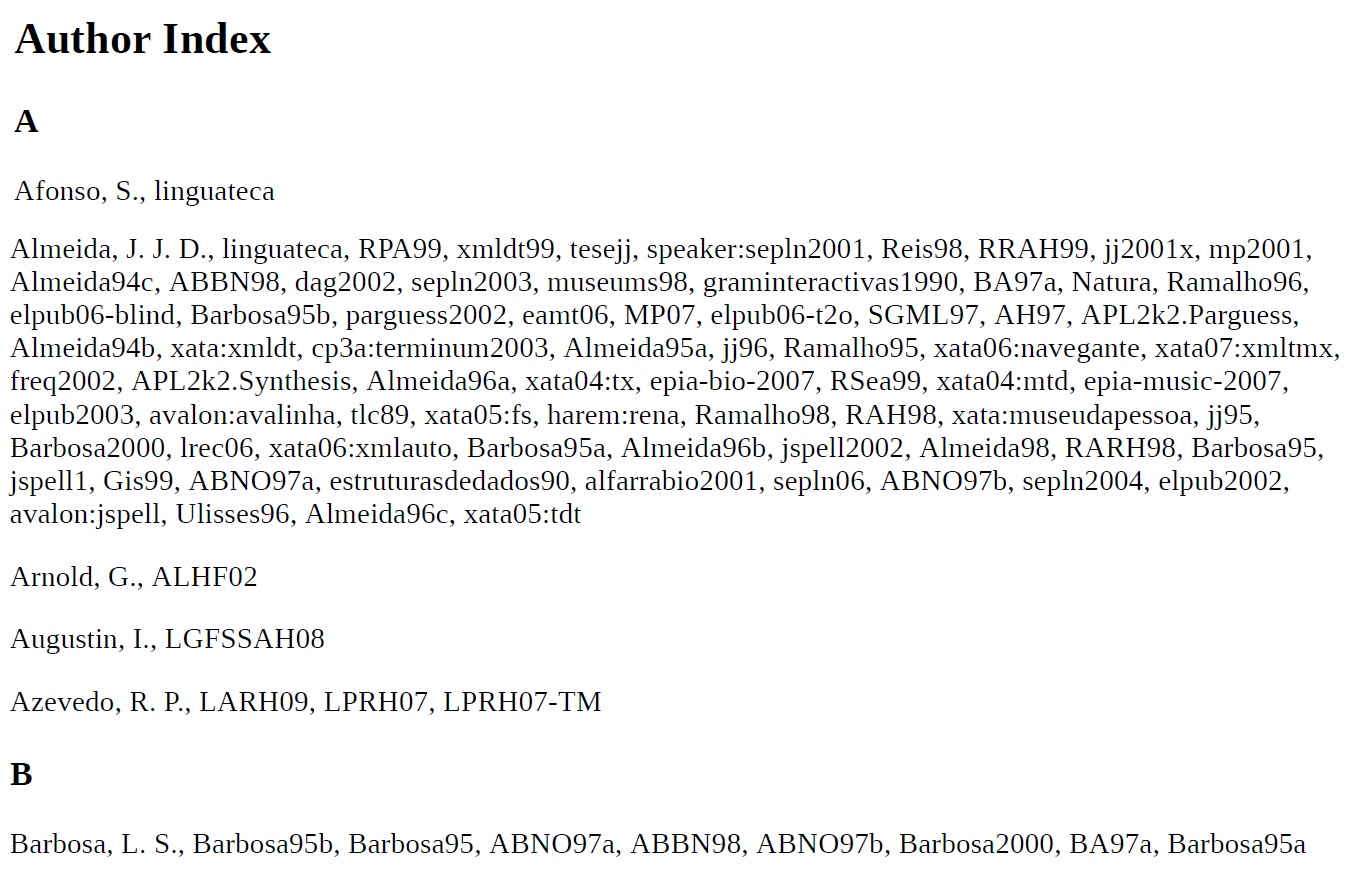
\includegraphics[width=1.2\textwidth]{P/authorIndex.jpeg}
\caption{Índice de Autores}
\end{figure}

\section{Tarefa 4 d}

\subsubsection{Implementação}
\begin{lstlisting}[language=python]
import os
import textwrap

def get_author_pub_graph(author,data):
    pub_partners = []
    for entry in data.values():
        if 'author' in entry and author in entry['author']:
            for partner in entry['author']:
                if partner != author:
                    pub_partners.append(partner)
    return [(author_name,pub_partners.count(author_name))
            for author_name in set(pub_partners)]


def get_dot_graph(author,data):
    g = sorted(get_author_pub_graph(author,data),key = lambda x: x[1])
    string_ls = ['graph{']
    string_ls2 = []
    for partner_author,no_joint_pub in g[-3:]:
        string_ls2.append(f'"{author}" -- "{partner_author}" [label="{no_joint_pub}"]')
    string_ls.append(textwrap.indent('\n'.join(string_ls2),'  '))
    string_ls.append('}')
    return '\n'.join(string_ls)

def get_html_dot_svg(author,data):
    DOT_INPUT_FILENAME = 'dot_input'
    with open(DOT_INPUT_FILENAME,'w') as file:
        file.write(get_dot_graph(author,data))
    os.system(f'dot -T svg -O {DOT_INPUT_FILENAME}')
    with open(DOT_INPUT_FILENAME + '.svg','r') as file:
        return re.search(r'<svg(?:.|\n)+</svg>',file.read()).group()

def get_html_common_pub_author(author,data):
    string_ls = [html_enclose('h2','Author Graph')]
    string_ls.append(get_html_dot_svg(author,data))
    return ''.join(string_ls)

\end{lstlisting}

\subsection{Resultado}
\begin{figure}[h]
\centering
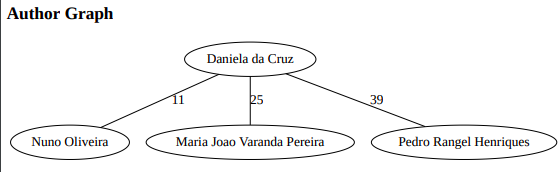
\includegraphics[width=1.5\textwidth]{P/authorGraph.jpeg}
\caption{Grafo de Autores}
\end{figure}


\chapter{Conclusão}
Através deste projeto foi possível expandir as nossas competências intelectuais sobre este tópico de estudo e, ao mesmo tempo, foi possível desenvolver as nossas aptidões enquanto grupo.


Assim, utilizando todos os nossos conhecimentos expostos neste trabalho e obtidos na sala de aula e é possível obter a tão esperada fotografia “perfeita”.


Concluindo este projeto, podemos afirmar que foi um trabalho muito
desafiante e enriquecedor para cada uma de nós, uma vez que tivemos a
oportunidade de explandir, aprofundar e aperfeiçoar os nossos conhecimentos
sobre a matéria lecionada na sala de aula e sobre a cinematografia. 
\appendix
\begin{appendices}
\chapter{Código do Programa}
De seguida lista-se o programa completo.
\begin{lstlisting}[language=python]
import re
import sys
import os
import os.path
import unicodedata

HTML_PROLOGUE = '<!DOCTYPE  html>\n<HTML lang="en">\n<HEAD>\n<meta charset="utf-8">\n      <TITLE>Categories in BibTeX</TITLE>\n <script type="text/x-mathjax-config"> MathJax.Hub.Config({"extensions":["tex2jax.js"],"jax":["input/TeX","output/HTML-CSS"],"messageStyle":"none","tex2jax":{"processEnvironments":false,"processEscapes":true,"inlineMath":[["$","$"]],"displayMath":[["$$","$$"],["\\[","\\]"]]},"TeX":{"extensions":["AMSmath.js","AMSsymbols.js","noErrors.js","noUndefined.js"]},"HTML-CSS":{"availableFonts":["TeX"]}}); </script> <script type="text/javascript" async src="file:////home/useralef/.vscode/extensions/shd101wyy.markdown-preview-enhanced-0.6.1/node_modules/@shd101wyy/mume/dependencies/mathjax/MathJax.js" charset="UTF-8"></script>  </HEAD>\n'
HTML_EPILOGUE = '</HTML>'
BIB_EXAMPLE_FILENAME = "exemplo-utf8.bib"
OUTPUT_FILENAME = 'output.html'

def get_bib_str(filename):
    with open(filename,'r') as file:
        return re.sub(r'\b}$',r' }',file.read())

def get_pub_type_counts(data):
    pub_types_occur = [x[0] for x in data.keys()]
    pub_types = set(pub_types_occur)
    return [(pub_type, pub_types_occur.count(pub_type)) for pub_type in pub_types]

def get_entries(string):
     d = {}
    field = re.compile(r'(\w+)\s*=\s*(?:{((?:[^{}]+|{(?:[^{}]+|{[^{}]*})+})+)}|"([^"]+)"|(\d+))')
    for entry in re.finditer(r"@(\w+){(.+),((?:[^{}]+|{(?:[^{}]*|{[^{}]*})+})+)", string):
        d[entry.group(1).lower(), entry.group(2)] = {
            x[0].lower(): get_valid_group(x, 1, 3)
            for x in field.findall(entry.group(3))}
    return d

def get_valid_group(t, begin_or_group, end_or_group):
    for i in range(begin_or_group, end_or_group + 1):
        if v := t[i]:
            return v

def unbrace(expression):
    return expression.translate({ord(x):None for x in '{}'})


def get_author_list(data):
    return sorted(set([a for s in data.values() for a in s.get("author", [])]))

def invert_name(author_name):
    return re.sub(r"([^,]+),\s*([^,]+)", r"\2 \1", author_name)

def remove_latex_special_chars(latex_expression):
    return re.sub(r'\\({|[^{])\b',r'\1',latex_expression)

def str_to_html_small_caps(expression):
    return html_to_small_caps(html_create_span(expression))

def html_create_span(expression):
    return html_enclose('span',expression)

def html_enclose(tag,string):
    return rf'<{tag.upper()}>{string}</{tag.upper()}>'

def html_to_small_caps(html_expression):
    return html_add_attr('style','font-variant:small-caps',html_expression)

def html_to_sans_serif(html_expression):
    return html_add_attr('style','font-family:sans-serif',html_expression)

def html_add_attr(attr,val,html_expression):
    return re.sub(r'<(\w+)([^>]*)\s*>(.*)</\1>',rf'<\1\2 {attr.upper()}="{val}">\3</\1>',html_expression)

def get_html_pub_type_index(data):
    string_ls = [html_enclose('h2','Publication Type Index')]
    for entry_type in sorted(set(x[0] for x in data)):
        string_ls.append(html_enclose('h3',entry_type))
        for citation_key in [x[1] for x in data if x[0]==entry_type]:
            title = data[entry_type,citation_key].get('title','')
            authors = ', '.join((sorted(data[entry_type,citation_key].get('author',''))))
            string_ls.append(html_enclose('p',f"Key = {citation_key}<br>Title = {fix_title(title)}<br>Autores = {authors}"))
    return '\n'.join(string_ls)

def str_to_html_math(string):
    return html_add_attr('class','math inline',html_create_span(string))

def fix_title(title):
    substitutions = [(r'\\textsc{((?:\\{|[^{])+)}',lambda m: f'{html_to_small_caps(html_create_span(m.group(1)))}'),
                     (r'\\textsf{((?:\\{|[^{])+)}',lambda m: f'{html_to_sans_serif(html_create_span(m.group(1)))}'),
                     (r'(\$(?:.|\\\$)+\$)', lambda m: f'{str_to_html_math(m.group(1))}')]


    replace = lambda x: mult_replace(x,substitutions)

    return   html_create_span(
             unbrace(
             replace(
             remove_latex_special_chars(
             ' '.join(s.strip() for s in title.split('\n'))))))


def mult_replace(string, replacement_list):
    for old, new in replacement_list:
        string = re.sub(old, new, string)
    return string

def fix_repeated_authors(data):
    author_blocks = fix_block_func(block_authors_with_two_common_names_v2(get_author_list(data)))
    author_dict = {author_name:max(s,key=len) for s in author_blocks for author_name in s}
    for d in data.values():
        d['author'] = [author_dict[author] for author in d['author']]

def format_authors(data):
    for d in data.values():
        if "author" in d:
            author_lst = [ remove_consecutive_spaces(
                           str.strip(
                           invert_name(
                           unbrace(
                           remove_accents(name)))))
                           for name in re.split(r"\band\b", d["author"].replace("\n", " "))]
            d['author'] = [author for author in author_lst if author]


def remove_consecutive_spaces(name):
    return re.sub(r'\s+',' ',name)

def remove_accents(name):
    return remove_latex_accent(remove_normal_accent(name))

def remove_latex_accent(name):
    return re.sub(r'\\\W','',name)

def remove_normal_accent(name):
    return ''.join((c for c in unicodedata.normalize('NFD', name) if unicodedata.category(c) != 'Mn'))

def last_name_first(name):
    initials =  '. '.join(get_crude_abbrev(name))[:-2]
    last_name = name.split()[-1]
    return f'{last_name}, {initials}'


def get_author_index_dict(data):
    index = {}
    for key, e in data.items():
        if 'author' in e:
            for author in e['author']:
                author_name = last_name_first(author)
                if author_name not in index:
                    index[author_name] = set()
                index[author_name].add(key[1])
    return index

def get_author_pub_graph(author,data):
    pub_partners = []
    for entry in data.values():
        if 'author' in entry and author in entry['author']:
            for partner in entry['author']:
                if partner != author:
                    pub_partners.append(partner)
    return [(author_name,pub_partners.count(author_name))
            for author_name in set(pub_partners)]

def get_html_author_index(data):
    index = sorted(get_author_index_dict(data).items())
    alphabet_order = sorted(set(c[0][0] for c in index))
    string_ls = [html_enclose('h2','Author Index')]
    i = 0
    string_ls.append(html_enclose('h3',alphabet_order[i]))
    for author,citation_keys in index:
        if author[0] != alphabet_order[i]:
            i += 1
            string_ls.append(html_enclose('h3',alphabet_order[i]))
        citation_keys_str = ', '.join(citation_keys)
        string_ls.append(html_enclose('p',f'{author}, {citation_keys_str}'))
    return ''.join(string_ls)


def get_crude_abbrev(name):
    return ''.join(c for c in name if c.isupper())


def is_a_first_last_match(author1,author2):
    a1 = get_crude_abbrev(author1)
    a2 = get_crude_abbrev(author2)
    return a1[0] == a2[0] and a1[-1] == a2[-1]

def block_authors_with_two_common_names(authors):
    res = set()
    for author in authors:
        fs = set()
        for author2 in authors:
            if len(set(re.findall(r'\w\w+',author)).intersection(re.findall(r'\w\w+',author2))) > 1:
                fs.add(author2)
        if not fs:
            print(author)
        res.add(frozenset(fs))
    return res

def block_authors_with_two_common_names_v2(authors):
    res = set()
    for author in authors:
        fs = set()
        for author2 in authors:
            a1 = set(re.findall(r'\w\w+',author))
            a2 = set(re.findall(r'\w\w+',author2))
            if len(a1.intersection(a2)) > 1:
                fs.add(author2)
            elif len(a1) == 1 and len(a1.intersection(a2)) == 1 and is_a_first_last_match(author,author2):
                fs.add(author2)
        res.add(frozenset(fs))
    return res

def fix_block_func(data):
    res = set()
    for s1 in data:
        q = s1.copy()
        for s2 in data:
            if s1.intersection(s2) != set():
                q = q.union(s2)
        res.add(frozenset(q))
    return res


def get_dot_graph(author,data):
    import textwrap
    g = sorted(get_author_pub_graph(author,data),key = lambda x: x[1])
    string_ls = ['graph{']
    string_ls2 = []
    for partner_author,no_joint_pub in g[-3:]:
        string_ls2.append(f'"{author}" -- "{partner_author}" [label="{no_joint_pub}"]')
    string_ls.append(textwrap.indent('\n'.join(string_ls2),'  '))
    string_ls.append('}')
    return '\n'.join(string_ls)


def get_html_pub_type_counts(data):
    string_ls = [html_enclose('h2','Number of Occurrences of Publication Types')]
    pub_counts = sorted(get_pub_type_counts(data),key=lambda x: x[1],reverse=True)
    time = lambda v: 's' if v > 1 else ''
    for pub_type, count in pub_counts:
        string_ls.append(html_enclose('p',f'Type {pub_type} appears {count} time{time(count)}'))
    return ''.join(string_ls)

def get_html_dot_svg(author,data):
    DOT_INPUT_FILENAME = 'dot_input'
    with open(DOT_INPUT_FILENAME,'w') as file:
        file.write(get_dot_graph(author,data))
    os.system(f'dot -T svg -O {DOT_INPUT_FILENAME}')
    with open(DOT_INPUT_FILENAME + '.svg','r') as file:
        return re.search(r'<svg(?:.|\n)+</svg>',file.read()).group()


def get_html_common_pub_author(author,data):
    string_ls = [html_enclose('h2','Author Graph')]
    string_ls.append(get_html_dot_svg(author,data))
    return ''.join(string_ls)

def solve(author_name,INPUT_FILENAME=BIB_EXAMPLE_FILENAME):
    html_str_ls = [HTML_PROLOGUE]
    bib_str = get_bib_str(INPUT_FILENAME)

    entries = get_entries(bib_str)
    format_authors(entries)
    fix_repeated_authors(entries)

    html_str_ls.append(html_enclose('body',f'{get_html_pub_type_counts(entries)}{get_html_common_pub_author(author_name,entries)}{get_html_pub_type_index(entries)}{get_html_author_index(entries)}'))

    html_str_ls.append(HTML_EPILOGUE)

    with open(OUTPUT_FILENAME,'w') as file:
        file.write('\n'.join(html_str_ls))

\end{lstlisting}
\chapter{Código de \emph{Output} do \emph{DOT}}

Apresenta-se agora aquilo que é escrito no ficheiro \emph{dot\_input}.

\begin{lstlisting}
graph{
  "Daniela da Cruz" -- "Nuno Oliveira" [label="11"]
  "Daniela da Cruz" -- "Maria Joao Varanda Pereira" [label="25"]
  "Daniela da Cruz" -- "Pedro Rangel Henriques" [label="39"]
}
\end{lstlisting}
\chapter{Código do \emph{Output} \emph{HTML}}

Apresenta-se agora aquilo que é escrito no ficheiro \emph{Output.html}.

\begin{lstlisting}
<!DOCTYPE  html>
<HTML lang="en">
<HEAD>
<meta charset="utf-8">
      <TITLE>Categories in BibTeX</TITLE>
 <script type="text/x-mathjax-config"> MathJax.Hub.Config({"extensions":["tex2jax.js"],"jax":["input/TeX","output/HTML-CSS"],"messageStyle":"none","tex2jax":{"processEnvironments":false,"processEscapes":true,"inlineMath":[["$","$"]],"displayMath":[]},"TeX":{"extensions":["AMSmath.js","AMSsymbols.js","noErrors.js","noUndefined.js"]},"HTML-CSS":{"availableFonts":["TeX"]}}); </script> <script type="text/javascript" async src="file:////home/useralef/.vscode/extensions/shd101wyy.markdown-preview-enhanced-0.6.1/node_modules/@shd101wyy/mume/dependencies/mathjax/MathJax.js" charset="UTF-8"></script>  </HEAD>

<BODY><H2>Number of Occurrences of Publication Types</H2><P>Type inproceedings appears 112 times</P><P>Type article appears 33 times</P><P>Type techreport appears 11 times</P><P>Type incollection appears 5 times</P><P>Type phdthesis appears 1 time</P><P>Type book appears 1 time</P><P>Type mastersthesis appears 1 time</P><P>Type misc appears 1 time</P><H2>Author Graph</H2><svg width="578pt" height="131pt"
 viewBox="0.00 0.00 577.59 131.00" xmlns="http://www.w3.org/2000/svg" xmlns:xlink="http://www.w3.org/1999/xlink">
<g id="graph0" class="graph" transform="scale(1 1) rotate(0) translate(4 127)">
<polygon fill="white" stroke="transparent" points="-4,4 -4,-127 573.59,-127 573.59,4 -4,4"/>
<!-- Daniela da Cruz -->
<g id="node1" class="node">
<title>Daniela da Cruz</title>
<ellipse fill="none" stroke="black" cx="249.74" cy="-105" rx="68.49" ry="18"/>
<text text-anchor="middle" x="249.74" y="-101.3" font-family="Times,serif" font-size="14.00">Daniela da Cruz</text>
</g>
<!-- Nuno Oliveira -->
<g id="node2" class="node">
<title>Nuno Oliveira</title>
<ellipse fill="none" stroke="black" cx="61.74" cy="-18" rx="61.99" ry="18"/>
<text text-anchor="middle" x="61.74" y="-14.3" font-family="Times,serif" font-size="14.00">Nuno Oliveira</text>
</g>
<!-- Daniela da Cruz&#45;&#45;Nuno Oliveira -->
<g id="edge1" class="edge">
<title>Daniela da Cruz&#45;&#45;Nuno Oliveira</title>
<path fill="none" stroke="black" d="M217,-89.19C182.39,-73.55 128.15,-49.02 93.8,-33.49"/>
<text text-anchor="middle" x="174.74" y="-57.8" font-family="Times,serif" font-size="14.00">11</text>
</g>
<!-- Maria Joao Varanda Pereira -->
<g id="node3" class="node">
<title>Maria Joao Varanda Pereira</title>
<ellipse fill="none" stroke="black" cx="249.74" cy="-18" rx="108.58" ry="18"/>
<text text-anchor="middle" x="249.74" y="-14.3" font-family="Times,serif" font-size="14.00">Maria Joao Varanda Pereira</text>
</g>
<!-- Daniela da Cruz&#45;&#45;Maria Joao Varanda Pereira -->
<g id="edge2" class="edge">
<title>Daniela da Cruz&#45;&#45;Maria Joao Varanda Pereira</title>
<path fill="none" stroke="black" d="M249.74,-86.8C249.74,-72.05 249.74,-50.92 249.74,-36.18"/>
<text text-anchor="middle" x="256.74" y="-57.8" font-family="Times,serif" font-size="14.00">25</text>
</g>
<!-- Pedro Rangel Henriques -->
<g id="node4" class="node">
<title>Pedro Rangel Henriques</title>
<ellipse fill="none" stroke="black" cx="472.74" cy="-18" rx="96.68" ry="18"/>
<text text-anchor="middle" x="472.74" y="-14.3" font-family="Times,serif" font-size="14.00">Pedro Rangel Henriques</text>
</g>
<!-- Daniela da Cruz&#45;&#45;Pedro Rangel Henriques -->
<g id="edge3" class="edge">
<title>Daniela da Cruz&#45;&#45;Pedro Rangel Henriques</title>
<path fill="none" stroke="black" d="M286.82,-89.87C326.95,-74.57 390.74,-50.26 432.18,-34.46"/>
<text text-anchor="middle" x="381.74" y="-57.8" font-family="Times,serif" font-size="14.00">39</text>
</g>
</g>
</svg><H2>Publication Type Index</H2>
<H3>article</H3>
<P>Key = jj96<br>Title = <SPAN>NLlex -- a tool to generate lexical analysers for natural language</SPAN><br>Autores = Jose Joao Dias de Almeida</P>
<P>Key = Ramalho98<br>Title = <SPAN>Algebraic specification of documents</SPAN><br>Autores = Jose Carlos Ramalho, Jose Joao Dias de Almeida, Pedro Rangel Henriques</P>
<P>Key = RRAH99<br>Title = <SPAN>SGML documents: Where does quality go?</SPAN><br>Autores = Jorge Gustavo Rocha, Jose Carlos Ramalho, Jose Joao Dias de Almeida, Pedro Rangel Henriques</P>
<P>Key = speaker:sepln2001<br>Title = <SPAN>Text to speech -- a rewriting system approach</SPAN><br>Autores = Alberto Manuel Brandao Simoes, Jose Joao Dias de Almeida</P>
<P>Key = parguess2002<br>Title = <SPAN>Grabbing parallel corpora from the web</SPAN><br>Autores = Alberto Manuel Brandao Simoes, J. Alves de Castro, Jose Joao Dias de Almeida</P>
<P>Key = sepln2003<br>Title = <SPAN>NATools -- A Statistical Word Aligner Workbench</SPAN><br>Autores = Alberto Manuel Brandao Simoes, Jose Joao Dias de Almeida</P>
<P>Key = xmldt2<br>Title = <SPAN>- Down-Translating XML</SPAN><br>Autores = Alberto Manuel Brandao Simoes</P>
<P>Key = sepln2004<br>Title = <SPAN>Distributed Translation Memories implementation using WebServices</SPAN><br>Autores = Alberto Manuel Brandao Simoes, Jose Joao Dias de Almeida, Xavier Gomez Guinovart</P>
<P>Key = sepln06<br>Title = <SPAN>A Client-Server Architecture for building Parallel Corpora applications</SPAN><br>Autores = Alberto Manuel Brandao Simoes, Jose Joao Dias de Almeida</P>
<P>Key = KMHVZ04<br>Title = <SPAN>Grammatical Approach to Problem Solving</SPAN><br>Autores = Maria Joao Varanda Pereira, Marjan Mernik, Pedro Rangel Henriques, Tomaz Kosar, Viljem Zumer</P>
<P>Key = HVMLGW05<br>Title = <SPAN>Automatic Generation of Language-based Tools using LISA System</SPAN><br>Autores = Hui Wu, Jeff Gray, Maria Joao Varanda Pereira, Marjan Mernik, Mitja Lenic, Pedro Rangel Henriques</P>
<P>Key = RMHV06<br>Title = <SPAN>AspectLISA: an aspect-oriented compiler construction system based on attribute grammars</SPAN><br>Autores = Damijan Rebernak, Maria Joao Varanda Pereira, Marjan Mernik, Pedro Rangel Henriques</P>
<P>Key = RMHCV06<br>Title = <SPAN>Specifying Languages using aspect-oriented approach: AspectLISA</SPAN><br>Autores = Damijan Rebernak, Daniela da Cruz, Maria Joao Varanda Pereira, Marjan Mernik, Pedro Rangel Henriques</P>
<P>Key = GDH06<br>Title = <SPAN>AG-based interactive system to retrieve information from XML documents</SPAN><br>Autores = Alda Lopes Gancarski, Anne Doucet, Pedro Rangel Henriques</P>
<P>Key = BH98<br>Title = <SPAN>A Framework and Patterns for the   Specification of Reactive Systems</SPAN><br>Autores = Leonor Barroca, Pedro Rangel Henriques</P>
<P>Key = RAH98<br>Title = <SPAN>Algebraic Specification of Documents</SPAN><br>Autores = Jose Carlos Ramalho, Jose Joao Dias de Almeida, Pedro Rangel Henriques</P>
<P>Key = RARH98<br>Title = <SPAN>SGML Documents: Where does quality go?</SPAN><br>Autores = Jorge Gustavo Rocha, Jose Carlos Ramalho, Jose Joao Dias de Almeida, Pedro Rangel Henriques</P>
<P>Key = GRH06<br>Title = <SPAN>Metamorphosis - A Topic Maps Based Environment to Handle Heterogeneous Information Resources</SPAN><br>Autores = Giovani Rubert Librelotto, Jose Carlos Ramalho, Pedro Rangel Henriques</P>
<P>Key = JGRH04<br>Title = <SPAN>XCSL Tutorial</SPAN><br>Autores = Giovani Rubert Librelotto, Jose Carlos Ramalho, Marta Jacinto, Pedro Rangel Henriques</P>
<P>Key = JGRH03<br>Title = <SPAN>XCSL: XML Constraint Specification Language</SPAN><br>Autores = Giovani Rubert Librelotto, Jose Carlos Ramalho, Marta Jacinto, Pedro Rangel Henriques</P>
<P>Key = GRH04<br>Title = <SPAN>TM-Builder: An Ontology Builder based on XML Topic Maps</SPAN><br>Autores = Giovani Rubert Librelotto, Jose Carlos Ramalho, Pedro Rangel Henriques</P>
<P>Key = GRH05a<br>Title = <SPAN>Geração automática de interfaces Web para Sistemas de Informação: Metamorphosis</SPAN><br>Autores = Giovani Rubert Librelotto, Jose Carlos Ramalho, Pedro Rangel Henriques</P>
<P>Key = RH98a<br>Title = <SPAN>Qualidade na Publicação Electrónica: como controlá-la?</SPAN><br>Autores = Jose Carlos Ramalho, Pedro Rangel Henriques</P>
<P>Key = MSH05<br>Title = <SPAN>Utilizando uma Base de Dados XML Nativa aplicada ao tratamento de erros num sistema de logs</SPAN><br>Autores = Giovana Mendes, Nuno Alberto Silva, Pedro Rangel Henriques</P>
<P>Key = ALHF02<br>Title = <SPAN>O Uso da Linguagem RS em Robótica</SPAN><br>Autores = Giovani Rubert Librelotto, Gustavo Arnold, Jaime Fonseca, Pedro Rangel Henriques</P>
<P>Key = CHV08ja<br>Title = <SPAN>Alma versus DDD</SPAN><br>Autores = Daniela da Cruz, Maria Joao Varanda Pereira, Pedro Rangel Henriques</P>
<P>Key = FPCH08jb<br>Title = <SPAN>Language in a Model-Based Engineering Environment for Control Systems -- An Approach for Compiler Implementation</SPAN><br>Autores = Daniela da Cruz, Elisabete Ferreira, Pedro Rangel Henriques, Rogerio Paulo</P>
<P>Key = PMCH08j<br>Title = <SPAN>Program Comprehension for Domain-Specific Languages (invited paper)</SPAN><br>Autores = Daniela da Cruz, Maria Joao Varanda Pereira, Marjan Mernik, Pedro Rangel Henriques</P>
<P>Key = CHV07<br>Title = <SPAN>Constructing program animations using a pattern-based approach</SPAN><br>Autores = Daniela da Cruz, Maria Joao Varanda Pereira, Pedro Rangel Henriques</P>
<P>Key = LARH09<br>Title = <SPAN>Topic Maps Constraint Languages: understanding and comparing</SPAN><br>Autores = Giovani Rubert Librelotto, Jose Carlos Ramalho, Pedro Rangel Henriques, Renato Preigschadt de Azevedo</P>
<P>Key = CBHP09<br>Title = <SPAN>Code Inspection Approaches for Program Visualization</SPAN><br>Autores = Daniela da Cruz, Maria Joao Varanda Pereira, Mario Beron, Pedro Rangel Henriques</P>
<P>Key = OPHCC2010<br>Title = <SPAN>VisualLISA: A Visual Environment to Develop Attribute Grammars</SPAN><br>Autores = Bastian Cramer, Daniela da Cruz, Maria Joao Varanda Pereira, Nuno Oliveira, Pedro Rangel Henriques</P>
<P>Key = KOMPCCH2010<br>Title = <SPAN>Comparing General-Purpose and Domain-Specific Languages: An Empirical Study</SPAN><br>Autores = Daniela da Cruz, Maria Joao Varanda Pereira, Marjan Mernik, Matej Crepinsek, Nuno Oliveira, Pedro Rangel Henriques, Tomaz Kosar</P>
<H3>book</H3>
<P>Key = RH02<br>Title = <SPAN>XML \& XSL: da teoria à prática</SPAN><br>Autores = Jose Carlos Ramalho, Pedro Rangel Henriques</P>
<H3>incollection</H3>
<P>Key = avalon:jspell<br>Title = <SPAN>nas Morfolimpíadas</SPAN><br>Autores = Alberto Manuel Brandao Simoes, Jose Joao Dias de Almeida</P>
<P>Key = avalon:avalinha<br>Title = <SPAN>Avaliação de alinhadores</SPAN><br>Autores = Alberto Manuel Brandao Simoes, Jose Joao Dias de Almeida</P>
<P>Key = harem:rena<br>Title = <SPAN>- Reconhecedor de Entidades</SPAN><br>Autores = Jose Joao Dias de Almeida</P>
<P>Key = RRH02<br>Title = <SPAN>Data Reduction to Improve Knowledge Extraction</SPAN><br>Autores = Carlos Ramos, Maria de Fatima Rodrigues, Pedro Rangel Henriques</P>
<P>Key = ORH06<br>Title = <SPAN>Data Cleaning by Reusing Domain Knowledge</SPAN><br>Autores = Maria de Fatima Rodrigues, Paulo Oliveira, Pedro Rangel Henriques</P>
<H3>inproceedings</H3>
<P>Key = graminteractivas1990<br>Title = <SPAN>Mecanismos para Especificação e Prototipagem de Interfaces Utilizador-Sistema</SPAN><br>Autores = F. Mario Martins, Jose Joao Dias de Almeida, Pedro Rangel Henriques</P>
<P>Key = Almeida94b<br>Title = <SPAN>GPC -- a Tool for higher-order grammar specification</SPAN><br>Autores = Jose Joao Dias de Almeida</P>
<P>Key = Almeida95a<br>Title = <SPAN>YaLG -- extending DCG for natural language processing</SPAN><br>Autores = Jose Joao Dias de Almeida</P>
<P>Key = Almeida94c<br>Title = <SPAN>Jspell -- um módulo para análise léxica genérica de linguagem natural</SPAN><br>Autores = Jose Joao Dias de Almeida, Ulisses Pinto</P>
<P>Key = Ramalho95<br>Title = <SPAN>Algebraic Specification of Documents</SPAN><br>Autores = Jose Carlos Ramalho, Jose Joao Dias de Almeida, Pedro Rangel Henriques</P>
<P>Key = Almeida96a<br>Title = <SPAN>Especificação e tratamento de Dicionários</SPAN><br>Autores = Jose Joao Dias de Almeida</P>
<P>Key = Ulisses96<br>Title = <SPAN>Tratamento automático de termos compostos</SPAN><br>Autores = Jose Joao Dias de Almeida, Ulisses Pinto</P>
<P>Key = Almeida96b<br>Title = <SPAN>YaLG a tool for higher-order grammar specification</SPAN><br>Autores = J.B. Barros, Jose Joao Dias de Almeida</P>
<P>Key = Ramalho96<br>Title = <SPAN>Document Semantics: two approaches</SPAN><br>Autores = Jose Carlos Ramalho, Jose Joao Dias de Almeida, Pedro Rangel Henriques</P>
<P>Key = SGML97<br>Title = <SPAN>SGML Documents: where does quality go?</SPAN><br>Autores = Jorge Gustavo Rocha, Jose Carlos Ramalho, Jose Joao Dias de Almeida, Pedro Rangel Henriques</P>
<P>Key = Almeida98<br>Title = <SPAN>Programação de dicionários</SPAN><br>Autores = Jose Joao Dias de Almeida</P>
<P>Key = Reis98<br>Title = <SPAN>Etiquetador morfo-sintáctico para o Português</SPAN><br>Autores = Jose Joao Dias de Almeida, Ricardo Reis</P>
<P>Key = ABNO97a<br>Title = <SPAN><SPAN STYLE="font-variant:small-caps">Camila</SPAN>: Formal Software Engineering Supported by Functional Programming</SPAN><br>Autores = F.L. Neves, J.N. Oliveira, Jose Joao Dias de Almeida, L.S. Barbosa</P>
<P>Key = ABNO97b<br>Title = <SPAN><SPAN STYLE="font-variant:small-caps">Camila</SPAN>: Prototyping and Refinement of Constructive Specifications</SPAN><br>Autores = F.L. Neves, J.N. Oliveira, Jose Joao Dias de Almeida, L.S. Barbosa</P>
<P>Key = AH97<br>Title = <SPAN>Dynamic Dictionary = cooperative information sources</SPAN><br>Autores = Jose Joao Dias de Almeida, Pedro Rangel Henriques</P>
<P>Key = museums98<br>Title = <SPAN>Adapting Museum Structures for the Web: No Changes Needed!</SPAN><br>Autores = J.L. Faria, Jorge Gustavo Rocha, Jose Carlos Ramalho, Jose Joao Dias de Almeida, Mario Ricardo Henriques, Pedro Rangel Henriques</P>
<P>Key = ABBN98<br>Title = <SPAN>On The Development of <SPAN STYLE="font-variant:small-caps">Camila</SPAN></SPAN><br>Autores = J.B. Barros, Jose Joao Dias de Almeida, L.F. Neves, L.S. Barbosa</P>
<P>Key = Gis99<br>Title = <SPAN>Systems Development</SPAN><br>Autores = Ana Silva, Jorge Gustavo Rocha, Jose Joao Dias de Almeida, Mario Ricardo Henriques, Pedro Rangel Henriques</P>
<P>Key = RPA99<br>Title = <SPAN>Maps</SPAN><br>Autores = Jorge Gustavo Rocha, Jose Joao Dias de Almeida, Tiago Pedroso</P>
<P>Key = RSea99<br>Title = <SPAN>SIG</SPAN><br>Autores = Ana Silva, Jorge Gustavo Rocha, Jose Joao Dias de Almeida, Mario Ricardo Henriques, Pedro Rangel Henriques</P>
<P>Key = xmldt99<br>Title = <SPAN>a Perl Down-Translation module</SPAN><br>Autores = Jose Carlos Ramalho, Jose Joao Dias de Almeida</P>
<P>Key = Barbosa2000<br>Title = <SPAN>Polytypic Recursion Patterns</SPAN><br>Autores = J.B. Barros, Jose Joao Dias de Almeida, L.S. Barbosa</P>
<P>Key = jj2001x<br>Title = <SPAN>Smallbook -- comando para produção de livros em pequena escala</SPAN><br>Autores = Jose Joao Dias de Almeida</P>
<P>Key = mp2001<br>Title = <SPAN>-- Arquitectura</SPAN><br>Autores = Alberto Manuel Brandao Simoes, Jorge Gustavo Rocha, Jose Joao Dias de Almeida, Pedro Rangel Henriques, Sonia Moreira</P>
<P>Key = alfarrabio2001<br>Title = <SPAN>Alfarrábio: Adding value to an Heterogeneous Site Collection</SPAN><br>Autores = Alberto Manuel Brandao Simoes, Jorge Gustavo Rocha, Jose Joao Dias de Almeida, Pedro Rangel Henriques</P>
<P>Key = freq2002<br>Title = <SPAN>Cálculo de frequências de palavras para entradas de dicionários através do uso conjunto de analisadores morfológicos, taggers e corpora</SPAN><br>Autores = Alberto Manuel Brandao Simoes, Jose Joao Dias de Almeida, Paulo A. Rocha</P>
<P>Key = jspell2002<br>Title = <SPAN>Jspell.pm -- um módulo de análise morfológica para uso em processamento de linguagem natural</SPAN><br>Autores = Alberto Manuel Brandao Simoes, Jose Joao Dias de Almeida</P>
<P>Key = dag2002<br>Title = <SPAN>Directory Attribute Grammars</SPAN><br>Autores = Alberto Manuel Brandao Simoes, Jose Joao Dias de Almeida, Pedro Rangel Henriques</P>
<P>Key = elpub2002<br>Title = <SPAN>Library::* -- a toolkit for digital libraries</SPAN><br>Autores = Alberto Manuel Brandao Simoes, Jose Joao Dias de Almeida</P>
<P>Key = APL2k2.Parguess<br>Title = <SPAN>Extracção de corpora paralelo a partir da web: construção e disponibilização</SPAN><br>Autores = Alberto Manuel Brandao Simoes, J. Alves de Castro, Jose Joao Dias de Almeida</P>
<P>Key = APL2k2.Synthesis<br>Title = <SPAN>Geração de voz com sotaque</SPAN><br>Autores = Alberto Manuel Brandao Simoes, Jose Joao Dias de Almeida</P>
<P>Key = xata:xmldt<br>Title = <SPAN>Engenharia reversa de HTML usando tecnologia XML</SPAN><br>Autores = Alberto Manuel Brandao Simoes, Jose Joao Dias de Almeida</P>
<P>Key = xata:museudapessoa<br>Title = <SPAN>essoa</SPAN><br>Autores = Alberto Manuel Brandao Simoes, Jose Joao Dias de Almeida</P>
<P>Key = elpub2003<br>Title = <SPAN>Music publishing</SPAN><br>Autores = Alberto Manuel Brandao Simoes, Jose Joao Dias de Almeida</P>
<P>Key = cp3a:terminum2003<br>Title = <SPAN>Projecto TerminUM</SPAN><br>Autores = Alberto Manuel Brandao Simoes, Bruno Martins, J. Alves de Castro, Jose Joao Dias de Almeida, Paulo Silva</P>
<P>Key = cp3a:kvec2003<br>Title = <SPAN>Lingua-Biterm: um módulo Perl para extracção de terminologia bilingue</SPAN><br>Autores = Bruno Martins</P>
<P>Key = cp3a:natools2003<br>Title = <SPAN>Alinhamento de corpora paralelos</SPAN><br>Autores = Alberto Manuel Brandao Simoes</P>
<P>Key = xata04:tx<br>Title = <SPAN>baseada em tipos dinâmicos</SPAN><br>Autores = Alberto Manuel Brandao Simoes, Jose Joao Dias de Almeida</P>
<P>Key = xata04:mtd<br>Title = <SPAN>Memórias de Tradução Distribuídas</SPAN><br>Autores = Alberto Manuel Brandao Simoes, Jose Joao Dias de Almeida, Xavier Gomez Guinovart</P>
<P>Key = linguateca<br>Title = <SPAN>Linguateca: um centro de recursos distribuído para o processamento computacional da língua portuguesa</SPAN><br>Autores = Alberto Manuel Brandao Simoes, Ana Frankenberg-Garcia, Ana Pinto, Anabela Barreiro, Belinda Maia, Cristina Mota, Debora Oliveira, Diana Santos, Eckhard Bick, Elisabete Ranchhod, Jose Joao Dias de Almeida, Luis Cabral, Luis Costa, Luis Sarmento, Marcirio Chaves, Nuno Cardoso, Paulo A. Rocha, Rachel Aires, Rosario Silva, Rui Vilela, Susana Afonso</P>
<P>Key = xata05:fs<br>Title = <SPAN>Representação em XML da Floresta Sintáctica</SPAN><br>Autores = Alberto Manuel Brandao Simoes, Eckhard Bick, Jose Joao Dias de Almeida, Rui Vilela</P>
<P>Key = xata05:tdt<br>Title = <SPAN>Inferência de tipos em documentos XML</SPAN><br>Autores = Alberto Manuel Brandao Simoes, Jose Joao Dias de Almeida</P>
<P>Key = xata06:navegante<br>Title = <SPAN>Navegante: um proxy de ordem superior para navegação intusiva</SPAN><br>Autores = Alberto Manuel Brandao Simoes, Jose Joao Dias de Almeida</P>
<P>Key = xata06:xmlauto<br>Title = <SPAN>XML</SPAN><br>Autores = Alberto Manuel Brandao Simoes, Jose Joao Dias de Almeida</P>
<P>Key = eamt06<br>Title = <SPAN>Combinatory Examples Extraction for Machine Translation</SPAN><br>Autores = Alberto Manuel Brandao Simoes, Jose Joao Dias de Almeida</P>
<P>Key = lrec06<br>Title = <SPAN>--- Recycling Thesauri into a Multilingual Ontology</SPAN><br>Autores = Alberto Manuel Brandao Simoes, Jose Joao Dias de Almeida</P>
<P>Key = elpub06-t2o<br>Title = <SPAN>Publishing multilingual ontologies: a quick way of obtaining feedback</SPAN><br>Autores = Alberto Manuel Brandao Simoes, Jose Joao Dias de Almeida</P>
<P>Key = elpub06-blind<br>Title = <SPAN>Transcoding for Web Accessibility for the Blind: Semantics from Structure</SPAN><br>Autores = Alberto Manuel Brandao Simoes, Alexandre Carvalho, Antonio R. Fernandes, Jose Joao Dias de Almeida</P>
<P>Key = xata07:xmltmx<br>Title = <SPAN>--- Processamento de Memórias de Tradução de Grandes Dimensões</SPAN><br>Autores = Alberto Manuel Brandao Simoes, Jose Joao Dias de Almeida</P>
<P>Key = MP07<br>Title = <SPAN>Dependency Specification Language</SPAN><br>Autores = Alberto Manuel Brandao Simoes, Jose Joao Dias de Almeida, Ruben Fonseca</P>
<P>Key = epia-bio-2007<br>Title = <SPAN>An Ontology-Based Approach To Systems Biology Literature Retrieval and Processing</SPAN><br>Autores = Alberto Manuel Brandao Simoes, Analia Lourenco, Eugenio Ferreira, Isabel Rocha, Jose Joao Dias de Almeida, Miguel Rocha</P>
<P>Key = epia-music-2007<br>Title = <SPAN>Using Text Mining Techniques for Classical Music Scores Analysis</SPAN><br>Autores = Alberto Manuel Brandao Simoes, Analia Lourenco, Jose Joao Dias de Almeida</P>
<P>Key = HKMVZ03<br>Title = <SPAN>Grammatical Approach to Problem Solving</SPAN><br>Autores = Maria Joao Varanda Pereira, Marjan Mernik, Pedro Rangel Henriques, Tomaz Kosar, Viljem Zumer</P>
<P>Key = VH01<br>Title = <SPAN>Visualization / Animation of Programs based on Abstract Representations and Formal Mappings</SPAN><br>Autores = Maria Joao Varanda Pereira, Pedro Rangel Henriques</P>
<P>Key = VH02<br>Title = <SPAN>Automatic Generation of Language-based Tools</SPAN><br>Autores = Maria Joao Varanda Pereira, Marjan Mernik, Mitja Lenic, Pedro Rangel Henriques</P>
<P>Key = VH03<br>Title = <SPAN>Visualization / Animation of Programs in Alma: obtaining different results</SPAN><br>Autores = Maria Joao Varanda Pereira, Pedro Rangel Henriques</P>
<P>Key = RMHVC06<br>Title = <SPAN>Specifying Languages using Aspect-oriented Approach: AspectLISA</SPAN><br>Autores = Damijan Rebernak, Daniela da Cruz, Maria Joao Varanda Pereira, Marjan Mernik, Pedro Rangel Henriques</P>
<P>Key = BHVU07d<br>Title = <SPAN>PICS una Herramienta para la Comprensión e Inspección de Programas</SPAN><br>Autores = Maria Joao Varanda Pereira, Mario Beron, Pedro Rangel Henriques, Roberto Uzal</P>
<P>Key = BHVU07c<br>Title = <SPAN>Program Inspection to Incerconnect Behavioral and Operational View for Program Comprehension</SPAN><br>Autores = Maria Joao Varanda Pereira, Mario Beron, Pedro Rangel Henriques, Roberto Uzal</P>
<P>Key = BHVU07b<br>Title = <SPAN>Comprensi'on de Programas por Inspecci'on Visual y Animaci'on</SPAN><br>Autores = Maria Joao Varanda Pereira, Mario Beron, Pedro Rangel Henriques, Roberto Uzal</P>
<P>Key = BHVU07a<br>Title = <SPAN>Static and Dynamic Strategies to Understand C Programs by Code Annotation</SPAN><br>Autores = Maria Joao Varanda Pereira, Mario Beron, Pedro Rangel Henriques, Roberto Uzal</P>
<P>Key = CHLB07a<br>Title = <SPAN>O Sitio de Pico, Software Educativo para Crianças con Paralisia Cerebral</SPAN><br>Autores = Elisabete Cunha, Mario Beron, Pedro Rangel Henriques, Sandra Cristina Lopes</P>
<P>Key = BHVU06a<br>Title = <SPAN>Herramientas para la compresión de programas</SPAN><br>Autores = Maria Joao Varanda Pereira, Mario Beron, Pedro Rangel Henriques, Roberto Uzal</P>
<P>Key = BHVU06b<br>Title = <SPAN>Comprensión de Algoritmos de Ruteo</SPAN><br>Autores = Maria Joao Varanda Pereira, Mario Beron, Pedro Rangel Henriques, Roberto Uzal</P>
<P>Key = BHVUM06<br>Title = <SPAN>A Language Processing Tool for Program Comprehension</SPAN><br>Autores = G. Montejano, Maria Joao Varanda Pereira, Mario Beron, Pedro Rangel Henriques, Roberto Uzal</P>
<P>Key = BHVU08<br>Title = <SPAN>Simplificando la Comprensión de Programas a través de la Interconnexión de Dominios</SPAN><br>Autores = Maria Joao Varanda Pereira, Mario Beron, Pedro Rangel Henriques, Roberto Uzal</P>
<P>Key = BHV06<br>Title = <SPAN>A System for Evaluate and Understand Routing Algorithms</SPAN><br>Autores = Maria Joao Varanda Pereira, Mario Beron, Pedro Rangel Henriques</P>
<P>Key = BCVHU08<br>Title = <SPAN>Evaluation Criteria of Software Visualization Systems used for Program Comprehension</SPAN><br>Autores = Daniela da Cruz, Maria Joao Varanda Pereira, Mario Beron, Pedro Rangel Henriques, Roberto Uzal</P>
<P>Key = BUHV08<br>Title = <SPAN>Inspección de Código para relacionar los Dominios del Problema y Programa para la Comprensión de Programas</SPAN><br>Autores = Maria Joao Varanda Pereira, Mario Beron, Pedro Rangel Henriques, Roberto Uzal</P>
<P>Key = OVH05<br>Title = <SPAN>Compreensão de Aplicações Web: O Processo e as Ferramentas</SPAN><br>Autores = Eva Oliveira, Maria Joao Varanda Pereira, Pedro Rangel Henriques</P>
<P>Key = OHV06<br>Title = <SPAN>Proposta de um Sistema para Compreensão de Aplicações Web</SPAN><br>Autores = Eva Oliveira, Maria Joao Varanda Pereira, Pedro Rangel Henriques</P>
<P>Key = GH07b<br>Title = <SPAN>Analyzing the structure of scientific articles to improve information retrieval</SPAN><br>Autores = Alda Lopes Gancarski, Pedro Rangel Henriques</P>
<P>Key = GH07a<br>Title = <SPAN>Using data together with metadata to improve XML information access</SPAN><br>Autores = Alda Lopes Gancarski, Pedro Rangel Henriques</P>
<P>Key = GFH08<br>Title = <SPAN>Using data together with metadata to improve XML information access</SPAN><br>Autores = Alda Lopes Gancarski, Flavio Xavier Ferreira, Pedro Rangel Henriques</P>
<P>Key = FGH08<br>Title = <SPAN>Information access from XML using semantics and context: application to the Portuguese Emigration Museum</SPAN><br>Autores = Alda Lopes Gancarski, Flavio Xavier Ferreira, Pedro Rangel Henriques</P>
<P>Key = FH08<br>Title = <SPAN>Using OWL to specify and build different views over the Emigration Museum resources</SPAN><br>Autores = Flavio Xavier Ferreira, Pedro Rangel Henriques</P>
<P>Key = LPRH07<br>Title = <SPAN>Navegando na Rede Semântica dos Topic Maps com o Ulisses</SPAN><br>Autores = Giovani Rubert Librelotto, Jose Carlos Ramalho, Pedro Rangel Henriques, Renato Preigschadt de Azevedo</P>
<P>Key = LPRH07-TM<br>Title = <SPAN>Topic Maps Constraint Specification Languages: comparing AsTMa!, OSL, and XTche</SPAN><br>Autores = Giovani Rubert Librelotto, Jose Carlos Ramalho, Pedro Rangel Henriques, Renato Preigschadt de Azevedo</P>
<P>Key = LRHGT08<br>Title = <SPAN>A Framework to specify, extract and manage Topic Maps driven by ontologie</SPAN><br>Autores = Giovani Rubert Librelotto, Jonas Bulegon Gassen, Jose Carlos Ramalho, Pedro Rangel Henriques, Rogerio Correa Turchetti</P>
<P>Key = LGFSSAH08<br>Title = <SPAN>Uma Ontologia aplicada a um Ambiente Pervasivo Hospitalar</SPAN><br>Autores = Fabio L. Silva, Giovani Rubert Librelotto, Iara Augustin, Jonas Bulegon Gassen, Leandro O. Freitas, Matheus C. Silveira, Pedro Rangel Henriques</P>
<P>Key = LMMVRH08<br>Title = <SPAN>Generating a Semantic Network for PubMed</SPAN><br>Autores = Giovani Rubert Librelotto, Henrique Machado, Jose Carlos Ramalho, Juliana Vizzotto, Mirkos Martins, Pedro Rangel Henriques</P>
<P>Key = CPH07f<br>Title = <SPAN>Pattern-based Program Visualization</SPAN><br>Autores = Daniela da Cruz, Maria Joao Varanda Pereira, Pedro Rangel Henriques</P>
<P>Key = CH07g<br>Title = <SPAN>Slicing wxHaskell modules to derive the User Interface Abstract Model (short paper and poster)</SPAN><br>Autores = Daniela da Cruz, Pedro Rangel Henriques</P>
<P>Key = CH07h<br>Title = <SPAN>Laboratory Site (poster)</SPAN><br>Autores = Daniela da Cruz, Pedro Rangel Henriques</P>
<P>Key = FCHV08<br>Title = <SPAN>How to interconnect operational and behavioral views of web applications</SPAN><br>Autores = Daniela da Cruz, Maria Joao Varanda Pereira, Pedro Rangel Henriques, Ruben Fonseca</P>
<P>Key = CHP08i<br>Title = <SPAN>Strategies for Program Inspection and Visualization</SPAN><br>Autores = Daniela da Cruz, Maria Joao Varanda Pereira, Pedro Rangel Henriques</P>
<P>Key = CH07a<br>Title = <SPAN>anguage</SPAN><br>Autores = Daniela da Cruz, Pedro Rangel Henriques</P>
<P>Key = CLH07c<br>Title = <SPAN>Como ensinar com Mapas de Conceitos: duas abordagens complementares</SPAN><br>Autores = Daniela da Cruz, Pedro Rangel Henriques, Sandra Cristina Lopes</P>
<P>Key = CH07d<br>Title = <SPAN>LISS --- The language and the compiler</SPAN><br>Autores = Daniela da Cruz, Pedro Rangel Henriques</P>
<P>Key = CFPBH07d<br>Title = <SPAN>Comparing Generators for Language-based Tools</SPAN><br>Autores = Daniela da Cruz, Maria Joao Varanda Pereira, Mario Beron, Pedro Rangel Henriques, Ruben Fonseca</P>
<P>Key = CHP08a<br>Title = <SPAN>Documents</SPAN><br>Autores = Daniela da Cruz, Maria Joao Varanda Pereira, Pedro Rangel Henriques</P>
<P>Key = CHP08b<br>Title = <SPAN>DDD</SPAN><br>Autores = Daniela da Cruz, Maria Joao Varanda Pereira, Pedro Rangel Henriques</P>
<P>Key = CPH08c<br>Title = <SPAN>Properties Preservation during Transformation (short paper)</SPAN><br>Autores = Daniela da Cruz, Jorge Sousa Pinto, Pedro Rangel Henriques</P>
<P>Key = FPCH08d<br>Title = <SPAN>Language in a Model-Based Engineering Environment for Control Systems --- An Approach for Compiler Implementation</SPAN><br>Autores = Daniela da Cruz, Elisabete Ferreira, Pedro Rangel Henriques, Rogerio Paulo</P>
<P>Key = PMCH08e<br>Title = <SPAN>: a Visual Interface for an Attribute Grammar based Compiler-Compiler (short paper)</SPAN><br>Autores = Daniela da Cruz, Maria Joao Varanda Pereira, Marjan Mernik, Pedro Rangel Henriques</P>
<P>Key = PMCH08f<br>Title = <SPAN>Program Comprehension for Domain-Specific Languages</SPAN><br>Autores = Daniela da Cruz, Maria Joao Varanda Pereira, Marjan Mernik, Pedro Rangel Henriques</P>
<P>Key = CHP09a<br>Title = <SPAN>Code Analysis: Past and Present</SPAN><br>Autores = Daniela da Cruz, Jorge Sousa Pinto, Pedro Rangel Henriques</P>
<P>Key = OPCH09a<br>Title = <SPAN>Visualization of Domain-Specific Programs' Behavior</SPAN><br>Autores = Daniela da Cruz, Maria Joao Varanda Pereira, Nuno Oliveira, Pedro Rangel Henriques</P>
<P>Key = oliveira09b<br>Title = <SPAN>Applying Program Comprehension Techniques to Karel Robot Programs</SPAN><br>Autores = Daniela da Cruz, Maria Joao Varanda Pereira, Marjan Mernik, Matej Crepinsek, Nuno Oliveira, Pedro Rangel Henriques, Tomaz Kosar</P>
<P>Key = oliveira09c<br>Title = <SPAN>VisualLISA: Visual Programming Environment for Attribute Grammars Specification</SPAN><br>Autores = Daniela da Cruz, Maria Joao Varanda Pereira, Nuno Oliveira, Pedro Rangel Henriques</P>
<P>Key = kosar09<br>Title = <SPAN>Influence of domain-specific notation to program understanding</SPAN><br>Autores = Daniela da Cruz, Maria Joao Varanda Pereira, Marjan Mernik, Nuno Oliveira, Pedro Rangel Henriques, Tomaz Kosar</P>
<P>Key = FCHGD09a<br>Title = <SPAN>A Query-by-Example Approach for XML Querying</SPAN><br>Autores = Alda Lopes Gancarski, Bruno Defude, Daniela da Cruz, Flavio Xavier Ferreira, Pedro Rangel Henriques</P>
<P>Key = ORH09a<br>Title = <SPAN>SMARTCLEAN: uma ferramenta para a limpeza incremental de dados</SPAN><br>Autores = Maria de Fatima Rodrigues, Paulo Jorge Oliveria, Pedro Rangel Henriques</P>
<P>Key = LPH09a<br>Title = <SPAN>Uma metodologia para Consultas aos Bancos de Dados do NCBI</SPAN><br>Autores = Giovani Rubert Librelotto, Pedro Rangel Henriques, Rafael Teodosio Pereira</P>
<P>Key = OPHC09a<br>Title = <SPAN>Domain Specific Languages: A Theoretical Survey</SPAN><br>Autores = Daniela da Cruz, Maria Joao Varanda Pereira, Nuno Oliveira, Pedro Rangel Henriques</P>
<P>Key = OPHCC09<br>Title = <SPAN>: A Domain Specific Visual Language for Attribute Grammars</SPAN><br>Autores = Bastian Cramer, Daniela da Cruz, Maria Joao Varanda Pereira, Nuno Oliveira, Pedro Rangel Henriques</P>
<P>Key = MKCHCPO09<br>Title = <SPAN>Comparison of XAML and C\# Forms using Cognitive Dimensions Framework</SPAN><br>Autores = Daniela da Cruz, Maria Joao Varanda Pereira, Marjan Mernik, Nuno Oliveira, Pedro Rangel Henriques, Tomaz Kosar</P>
<P>Key = OHCP09<br>Title = <SPAN>XAGra - An XML Dialect for Attribute Grammars</SPAN><br>Autores = Daniela da Cruz, Maria Joao Varanda Pereira, Nuno Oliveira, Pedro Rangel Henriques</P>
<P>Key = FCHGD09b<br>Title = <SPAN>GuessXQ, an inference Web-engine for querying XML Documents</SPAN><br>Autores = Alda Lopes Gancarski, Bruno Defude, Daniela da Cruz, Flavio Xavier Ferreira, Pedro Rangel Henriques</P>
<P>Key = BHVU09<br>Title = <SPAN>Instrumentaciones de Programas Escritos en C para Interrelacionar las Vistas Comportamental y Operacional de los Sistemas de Software</SPAN><br>Autores = Maria Joao Varanda Pereira, Mario Beron, Pedro Rangel Henriques, Roberto Uzal</P>
<P>Key = CH09d<br>Title = <SPAN>Assessing Databases in .Net: comparing approaches</SPAN><br>Autores = Daniela da Cruz, Pedro Rangel Henriques</P>
<P>Key = CH2010a<br>Title = <SPAN>Exploring, Visualizing and Slicing the Soul of XML Documents</SPAN><br>Autores = Daniela da Cruz, Pedro Rangel Henriques</P>
<H3>mastersthesis</H3>
<P>Key = teseambs<br>Title = <SPAN>Parallel Corpora word alignment and applications</SPAN><br>Autores = Alberto Manuel Brandao Simoes</P>
<H3>misc</H3>
<P>Key = cruz09<br>Title = <SPAN>GraAL - A Grammar Analyzer</SPAN><br>Autores = Daniela da Cruz, Nuno Oliveira, Pedro Rangel Henriques</P>
<H3>phdthesis</H3>
<P>Key = tesejj<br>Title = <SPAN>Dicionários dinâmicos multi-fonte</SPAN><br>Autores = Jose Joao Dias de Almeida</P>
<H3>techreport</H3>
<P>Key = tlc89<br>Title = <SPAN>Teoria das Linguagens</SPAN><br>Autores = J.B. Barros, Jose Joao Dias de Almeida</P>
<P>Key = estruturasdedados90<br>Title = <SPAN>Estruturas de Dados</SPAN><br>Autores = J.B. Barros, Jose Joao Dias de Almeida</P>
<P>Key = Camila<br>Title = <SPAN><SPAN STYLE="font-variant:small-caps">Camila</SPAN> - A Platform for Software Mathematical Development</SPAN><br>Autores = projecto Camila</P>
<P>Key = Natura<br>Title = <SPAN>Natura - Natural language processing</SPAN><br>Autores = Jose Joao Dias de Almeida</P>
<P>Key = jspell1<br>Title = <SPAN>Manual de Utilizador do JSpell</SPAN><br>Autores = Jose Joao Dias de Almeida, Ulisses Pinto</P>
<P>Key = jj95<br>Title = <SPAN>NLlex -- a tool to generate lexical analysers for natural language</SPAN><br>Autores = Jose Joao Dias de Almeida</P>
<P>Key = Barbosa95<br>Title = <SPAN>System Prototyping in <SPAN STYLE="font-variant:small-caps">Camila</SPAN></SPAN><br>Autores = Jose Joao Dias de Almeida, L.S. Barbosa</P>
<P>Key = Barbosa95a<br>Title = <SPAN><SPAN STYLE="font-variant:small-caps">Camila</SPAN>: A reference Manual</SPAN><br>Autores = Jose Joao Dias de Almeida, L.S. Barbosa</P>
<P>Key = BA97a<br>Title = <SPAN>Systems Prototyping in <SPAN STYLE="font-variant:small-caps">Camila</SPAN></SPAN><br>Autores = Jose Joao Dias de Almeida, L.S. Barbosa</P>
<P>Key = Barbosa95b<br>Title = <SPAN>Growing Up With <SPAN STYLE="font-variant:small-caps">Camila</SPAN></SPAN><br>Autores = Jose Joao Dias de Almeida, L.S. Barbosa</P>
<P>Key = Almeida96c<br>Title = <SPAN>From BiBTeX to HTML semantic nets</SPAN><br>Autores = Jose Carlos Ramalho, Jose Joao Dias de Almeida</P><H2>Author Index</H2><H3>A</H3><P>Afonso, S., linguateca</P><P>Aires, R., linguateca</P><P>Almeida, J. J. D., linguateca, RPA99, xmldt99, tesejj, speaker:sepln2001, Reis98, RRAH99, jj2001x, mp2001, Almeida94c, ABBN98, dag2002, sepln2003, museums98, graminteractivas1990, BA97a, Natura, Ramalho96, elpub06-blind, Barbosa95b, parguess2002, eamt06, MP07, elpub06-t2o, SGML97, AH97, APL2k2.Parguess, Almeida94b, xata:xmldt, cp3a:terminum2003, Almeida95a, jj96, Ramalho95, xata06:navegante, xata07:xmltmx, freq2002, APL2k2.Synthesis, Almeida96a, xata04:tx, epia-bio-2007, RSea99, xata04:mtd, epia-music-2007, elpub2003, avalon:avalinha, tlc89, xata05:fs, harem:rena, Ramalho98, RAH98, xata:museudapessoa, jj95, Barbosa2000, lrec06, xata06:xmlauto, Barbosa95a, Almeida96b, jspell2002, Almeida98, RARH98, Barbosa95, jspell1, Gis99, ABNO97a, estruturasdedados90, alfarrabio2001, sepln06, ABNO97b, sepln2004, elpub2002, avalon:jspell, Ulisses96, Almeida96c, xata05:tdt</P><P>Arnold, G., ALHF02</P><P>Augustin, I., LGFSSAH08</P><P>Azevedo, R. P., LARH09, LPRH07, LPRH07-TM</P><H3>B</H3><P>Barbosa, L. S., Barbosa95b, Barbosa95, ABNO97a, ABBN98, ABNO97b, Barbosa2000, BA97a, Barbosa95a</P><P>Barreiro, A., linguateca</P><P>Barroca, L., BH98</P><P>Barros, J. B., Almeida96b, estruturasdedados90, ABBN98, tlc89, Barbosa2000</P><P>Beron, M., BHVU08, BHVU07d, BCVHU08, BHVU07a, BHV06, BHVUM06, BHVU09, BHVU06b, BHVU07c, CBHP09, BHVU07b, BUHV08, BHVU06a, CFPBH07d, CHLB07a</P><P>Bick, E., linguateca, xata05:fs</P><H3>C</H3><P>Cabral, L., linguateca</P><P>Camila, , Camila</P><P>Cardoso, N., linguateca</P><P>Carvalho, A., elpub06-blind</P><P>Castro, J. A., cp3a:terminum2003, parguess2002, APL2k2.Parguess</P><P>Chaves, M., linguateca</P><P>Costa, L., linguateca</P><P>Cramer, B., OPHCC09, OPHCC2010</P><P>Crepinsek, M., KOMPCCH2010, oliveira09b</P><P>Cruz, D., FPCH08d, oliveira09b, KOMPCCH2010, RMHCV06, oliveira09c, CH07d, CHV07, PMCH08j, CLH07c, BCVHU08, FCHGD09a, FCHGD09b, cruz09, CH07h, CHV08ja, CHP09a, CFPBH07d, PMCH08e, CPH08c, CH07g, kosar09, CHP08a, OPHCC2010, CPH07f, RMHVC06, CBHP09, OPCH09a, FPCH08jb, CH2010a, CHP08b, CHP08i, OPHC09a, PMCH08f, MKCHCPO09, OHCP09, OPHCC09, CH09d, CH07a, FCHV08</P><P>Cunha, E., CHLB07a</P><H3>D</H3><P>Defude, B., FCHGD09a, FCHGD09b</P><P>Doucet, A., GDH06</P><H3>F</H3><P>Faria, J. L., museums98</P><P>Fernandes, A. R., elpub06-blind</P><P>Ferreira, E., epia-bio-2007, FPCH08d, FPCH08jb</P><P>Ferreira, F. X., FH08, FGH08, FCHGD09b, FCHGD09a, GFH08</P><P>Fonseca, J., ALHF02</P><P>Fonseca, R., MP07, FCHV08, CFPBH07d</P><P>Frankenberg-Garcia, A. F., linguateca</P><P>Freitas, L. O., LGFSSAH08</P><H3>G</H3><P>Gancarski, A. L., GH07b, GDH06, GH07a, FGH08, FCHGD09a, FCHGD09b, GFH08</P><P>Gassen, J. B., LGFSSAH08, LRHGT08</P><P>Gray, J., HVMLGW05</P><P>Guinovart, X. G., sepln2004, xata04:mtd</P><H3>H</H3><P>Henriques, M. R., RSea99, Gis99, museums98</P><P>Henriques, P. R., FPCH08d, ORH09a, HKMVZ03, JGRH03, cruz09, BH98, kosar09, PMCH08e, CPH08c, RMHVC06, RH98a, OPCH09a, BHVU07b, FPCH08jb, CHP08b, CHLB07a, OPHC09a, LRHGT08, Gis99, PMCH08f, MKCHCPO09, LMMVRH08, alfarrabio2001, LARH09, HVMLGW05, RMHV06, GH07a, oliveira09b, oliveira09c, dag2002, museums98, LGFSSAH08, CHV07, CLH07c, BCVHU08, AH97, GRH06, BHVU07c, Ramalho95, CFPBH07d, OPHCC2010, BHVU06a, GDH06, OHV06, RARH98, OHCP09, OPHCC09, CH09d, CH07a, FCHV08, OVH05, GFH08, MSH05, RRAH99, ALHF02, mp2001, CH07d, Ramalho96, graminteractivas1990, KMHVZ04, LPRH07, FH08, SGML97, RH02, RRH02, FCHGD09a, FCHGD09b, CH07h, BHVU08, GH07b, CH07g, VH01, LPH09a, BUHV08, GRH04, VH03, CHP08i, BHVU06b, JGRH04, LPRH07-TM, BHVU07d, KOMPCCH2010, GRH05a, RMHCV06, BHVUM06, VH02, PMCH08j, ORH06, BHVU09, CHV08ja, CHP09a, CHP08a, FGH08, RSea99, BHVU07a, CPH07f, CBHP09, Ramalho98, RAH98, CH2010a, BHV06</P><H3>J</H3><P>Jacinto, M., JGRH03, JGRH04</P><H3>K</H3><P>Kosar, T., oliveira09b, MKCHCPO09, KOMPCCH2010, HKMVZ03, KMHVZ04, kosar09</P><H3>L</H3><P>Lenic, M., VH02, HVMLGW05</P><P>Librelotto, G. R., LRHGT08, LPRH07, JGRH03, GRH05a, ALHF02, LMMVRH08, LPH09a, GRH06, LARH09, LGFSSAH08, JGRH04, GRH04, LPRH07-TM</P><P>Lopes, S. C., CLH07c, CHLB07a</P><P>Lourenco, A., epia-bio-2007, epia-music-2007</P><H3>M</H3><P>Machado, H., LMMVRH08</P><P>Maia, B., linguateca</P><P>Martins, B., cp3a:terminum2003, cp3a:kvec2003</P><P>Martins, F. M., graminteractivas1990</P><P>Martins, M., LMMVRH08</P><P>Mendes, G., MSH05</P><P>Mernik, M., PMCH08j, oliveira09b, PMCH08f, MKCHCPO09, KOMPCCH2010, RMHCV06, RMHVC06, HKMVZ03, HVMLGW05, VH02, RMHV06, KMHVZ04, kosar09, PMCH08e</P><P>Montejano, G., BHVUM06</P><P>Moreira, S., mp2001</P><P>Mota, C., linguateca</P><H3>N</H3><P>Neves, F. L., ABNO97b, ABNO97a</P><P>Neves, L. F., ABBN98</P><H3>O</H3><P>Oliveira, D., linguateca</P><P>Oliveira, E., OHV06, OVH05</P><P>Oliveira, J. N., ABNO97b, ABNO97a</P><P>Oliveira, N., OPHC09a, oliveira09b, MKCHCPO09, OHCP09, OPHCC2010, KOMPCCH2010, OPHCC09, oliveira09c, cruz09, OPCH09a, kosar09</P><P>Oliveira, P., ORH06</P><P>Oliveria, P. J., ORH09a</P><H3>P</H3><P>Paulo, R., FPCH08d, FPCH08jb</P><P>Pedroso, T., RPA99</P><P>Pereira, M. J. V., oliveira09b, BHVU07d, KOMPCCH2010, RMHCV06, oliveira09c, BHVUM06, HKMVZ03, VH02, KMHVZ04, CHV07, PMCH08j, BCVHU08, BHVU07c, BHVU09, CHV08ja, CFPBH07d, PMCH08e, BHVU08, kosar09, CHP08a, OPHCC2010, CPH07f, RMHVC06, VH01, BHVU07a, CBHP09, OPCH09a, BHVU07b, BUHV08, CHP08b, CHP08i, BHVU06a, VH03, OPHC09a, OHV06, PMCH08f, MKCHCPO09, OHCP09, OPHCC09, BHV06, FCHV08, BHVU06b, HVMLGW05, OVH05, RMHV06</P><P>Pereira, R. T., LPH09a</P><P>Pinto, A., linguateca</P><P>Pinto, J. S., CPH08c, CHP09a</P><P>Pinto, U., Ulisses96, Almeida94c, jspell1</P><H3>R</H3><P>Ramalho, J. C., xmldt99, RRAH99, GRH05a, Almeida96c, museums98, Ramalho96, LPRH07, JGRH03, SGML97, RH02, GRH06, Ramalho95, RH98a, Ramalho98, RAH98, GRH04, LRHGT08, RARH98, LMMVRH08, LARH09, JGRH04, LPRH07-TM</P><P>Ramos, C., RRH02</P><P>Ranchhod, E., linguateca</P><P>Rebernak, D., RMHVC06, RMHV06, RMHCV06</P><P>Reis, R., Reis98</P><P>Rocha, I., epia-bio-2007</P><P>Rocha, J. G., RPA99, RARH98, Gis99, RRAH99, RSea99, SGML97, mp2001, alfarrabio2001, museums98</P><P>Rocha, M., epia-bio-2007</P><P>Rocha, P. A., linguateca, freq2002</P><P>Rodrigues, M. F., ORH09a, ORH06, RRH02</P><H3>S</H3><P>Santos, D., linguateca</P><P>Sarmento, L., linguateca</P><P>Silva, A., RSea99, Gis99</P><P>Silva, F. L., LGFSSAH08</P><P>Silva, N. A., MSH05</P><P>Silva, P., cp3a:terminum2003</P><P>Silva, R., linguateca</P><P>Silveira, M. C., LGFSSAH08</P><P>Simoes, A. M. B., xmldt2, linguateca, speaker:sepln2001, mp2001, teseambs, dag2002, sepln2003, elpub06-blind, parguess2002, eamt06, MP07, elpub06-t2o, APL2k2.Parguess, xata:xmldt, cp3a:terminum2003, xata06:navegante, xata07:xmltmx, freq2002, APL2k2.Synthesis, xata04:tx, epia-bio-2007, xata04:mtd, epia-music-2007, cp3a:natools2003, elpub2003, avalon:avalinha, xata05:fs, xata:museudapessoa, xata06:xmlauto, jspell2002, alfarrabio2001, sepln06, sepln2004, elpub2002, avalon:jspell, lrec06, xata05:tdt</P><H3>T</H3><P>Turchetti, R. C., LRHGT08</P><H3>U</H3><P>Uzal, R., BHVU08, BHVU07d, BCVHU08, BHVU07a, BHVUM06, BHVU09, BHVU06b, BHVU07c, BHVU07b, BUHV08, BHVU06a</P><H3>V</H3><P>Vilela, R., linguateca, xata05:fs</P><P>Vizzotto, J., LMMVRH08</P><H3>W</H3><P>Wu, H., HVMLGW05</P><H3>Z</H3><P>Zumer, V., HKMVZ03, KMHVZ04</P></BODY>
</HTML>
\end{lstlisting}
\end{appendices} 

\end{document}
